\begin{frame} [Status] 
\frametitle{Status for week of \today}
\begin{enumerate} 
\item 
\item Setting up tools and git repo in prep for better collaboration
\end{enumerate}
\end{frame} 

\begin{frame} [Status] 
\frametitle{Status for advisor week of \today}
\begin{enumerate} 
\item Finishing slides for IPDPS. 
\item Discussion with Amanda: we are aiming to formalizing study, including putting an INCITE proposal. 
\item Finishing some runs with AMG. 
\item Setting up tools and git repo in prep for better collaboration. 
\end{enumerate}
\end{frame}  


\begin{frame}
\frametitle{Action Items}
\begin{enumerate}
\tiny \item \tiny  BlueWaters access?  This would allow us to have a comparison machine to Sequoia in our work. \\
\item \tiny Question about INCITE proposal with Amanda. This will be used as a mechanism to help formalize Amanda's collab with us.  \\
\item \tiny Considering applying to George Micheal award, Mark Hoemmen suggested I do this. 
 Wanted to know if this would work, and if I should do it.  \\
\end{enumerate}
\end{frame}  

\begin{frame} [Tasks] 
\frametitle{Task: Simulator setup and slack-conscious sched(Estimated time: 1 week to 1.5 weeks)}
\begin{enumerate} 
\item Make sure it works properly on laptop, write a readme for running. 
\item Incorporate slack-conscious scheduling
\item Experimentation with AMG applications 
\end{enumerate}
\end{frame}  

\begin{frame} [Tasks] 
\frametitle{Task: Tools setup(Estimated time: 4-5 days)}
\begin{enumerate} 
\item algo strategy software: library (linking+loading). \\
\item collaboration support:  git repo setup. \\
\item Publicizing: Doxygen + wiki + website. \\
\item Results organization:  gnuplot+graphing utils. \\
\end{enumerate}
\end{frame}  

\begin{frame} [Tasks] 
\frametitle{Task: Revise current Concepts/Theoretical Analysis (Est time: 3 days) }
\begin{enumerate} 
\item Theoretical Analysis: have simple version ready \\
\item Strategy Explanation: \\
\begin{itemize}
   \item diagrams of strategies. 
   \item  Patterns (get document in shape, and explain forces). 
\end{itemize} 
\end{enumerate}
\end{frame}  

\begin{frame} [Tasks] 
\frametitle{Task: Additional Experimentation on BG/Q and BW (Est time: 4 days)}
\begin{enumerate} 
\item do fully dynamic sched. 
\item check slack-conscious sched. 
\item do experimentation with different compilers. 
\item check experimentation with different system configuration settings. 
\end{enumerate} 
\end{frame}  

\begin{frame} [Tasks] 
\frametitle{Task: Risk Analysis (Est time:  4 days) }
\begin{enumerate} 
\item Review statistics and game theory. 
\item Look through noise theoretical work by Tsasfir.
\item connect game theory and statistic to noise, so that we 
can adjust static fraction for sched. 
\end{enumerate} 
\end{frame} 

\begin{frame}
\frametitle{Brainstorming}
\begin{columns} % contents are top vertically aligned 
\column{0.5\textwidth} 
\begin{itemize} 
\tiny \item \tiny Techniques: multi-stage scheduling.  \\
\item \tiny  Techniques: Hybrid blocking/non-blocking collectives.   \\
\item \tiny  Techniques: Within-timestep affinity adjusting scheduling    \\
 \item \tiny Techniques: Network topology conscious sched \\
\item \tiny Experimental design:  use noise injection instead of simulation. 
\end{itemize}
\column{0.5\textwidth} 
\end{columns} 
\end{frame} 

\begin{frame}
\frametitle{Schedule(Summer 2012)}
\begin{itemize}
\tiny \item \tiny May 13 - 22:  tools setup, software setup, IPDPS presentation, website setup. \\
\item \tiny May 22nd - June 3rd: Work on thesis, application of shared mem extensions in Amanda's code. \\
\item \tiny June 3rd - June 15th: Go through AMG perf model. \\
\item \tiny June 15th - July 15th: Risk Analysis tests with simple computation. \\ 
\item \tiny July 15th - Aug 15th: apply to real code. \\
\item \tiny Aug 15th - Sept 1st: gather results and do IPDPS write-up. \\
\end{itemize} 
\end{frame} 

\begin{frame} 
\frametitle{Schedule(Fall 2012)}
\begin{itemize}
\tiny \item \tiny Sept 1st - Oct 1st: IPDPS write-up for risk analysis .
\item \tiny Oct 1st - Dec 1st : Journal with Prof Grigori and Ulrike + MPI shared memory programming model + prelim  
\item \tiny Dec 1st - Jan 15th : organize code, thesis writing plan and organization
\item \tiny Jan 15th - May 15th : thesis writing ,  Gordon Bell submission or SC submission for LBM work.   
\end{itemize} 
\end{frame} 

\begin{frame}  
\frametitle{Solution Summary} 
\begin{columns}
\column{0.33\textwidth} 
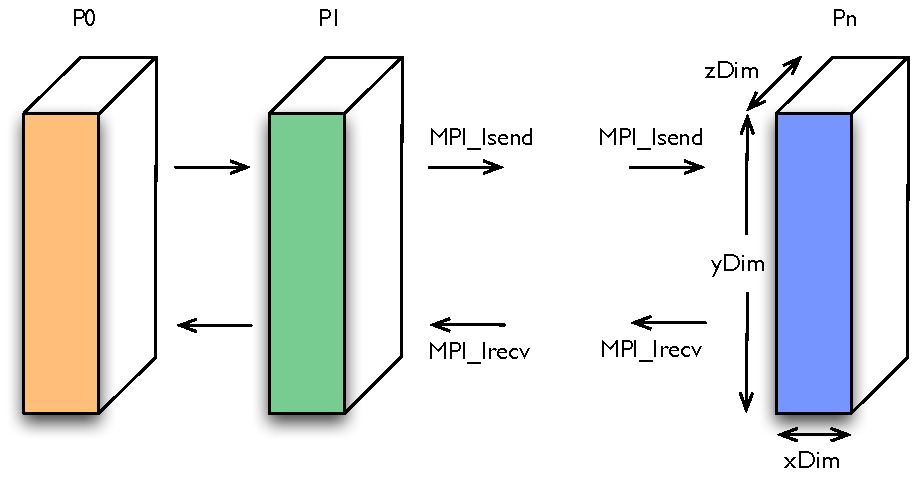
\includegraphics[width=\textwidth]{images/mpi_decomp}
Original 
\column{0.33\textwidth}
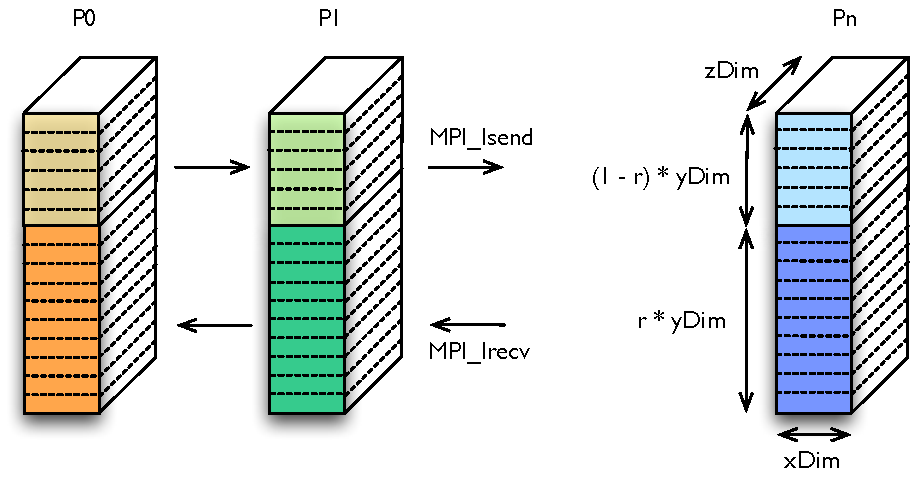
\includegraphics[width=\textwidth]{images/hybrid_decomp}
$\mu$-sched 
\column{0.33\textwidth}
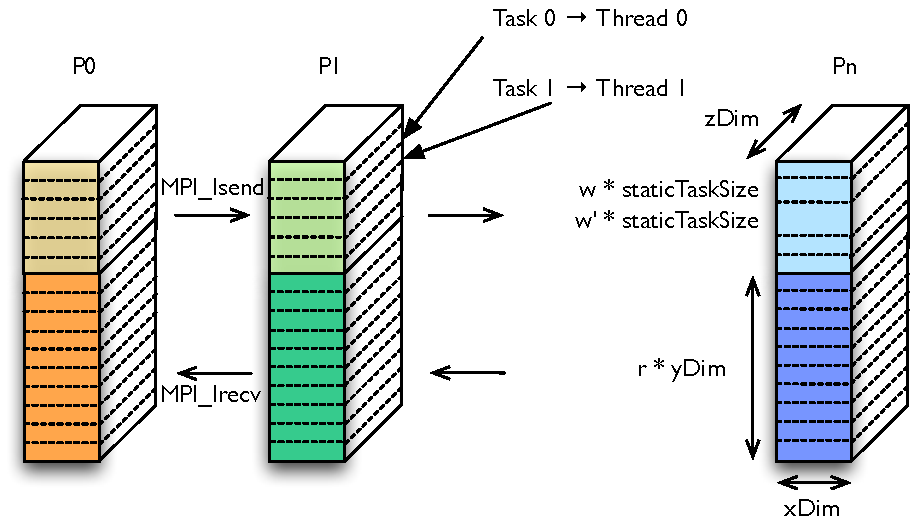
\includegraphics[width=\textwidth]{images/weighted_decomp}
Weighted $\mu$-sched 
\end{columns}
\end{frame}  

\begin{frame}[Discussion]
\frametitle{Discussion} 
\begin{itemize}
\item \small Architectures may advance yearly, but remember that OS is changing and advancing also.
\item \small Operating system may have been programmed 
inefficiently, creating larger overheads than 
one would expect. The net effect of inefficient
programming of Operating System is again more OS noise. 
\item \small  The ``noise'' \textit{does not just come from the OS}; it 
can also come from hardware variations, app load imbalance, runtime, 
interaction between app and runtime, hybridized runtimes, ... \\  
\item \small To statically parallelize the entire
hardware/software stack is very difficult, and so an adaptive, lightweight scheduling
seems to be the right solution to scale past the noise amplification problem
(and works with good success, as our results show). 
\end{itemize}
\end{frame}


\begin{frame}[Related Work] 
\frametitle{Related Work}
\begin{enumerate}
\item Work-stealing with Trim Analysis 
\item PLASMA and DPLASMA 
\item Periodic load balancing
\item Co-scheduling
\item FASTOS
\item Tesselation 
\end{enumerate} 
\end{frame} 


\begin{frame}[Theoretical Analysis]
\frametitle{Theoretical Analysis of Lightweight Scheduling}
\begin{itemize}
\item \tiny Let $t = T_p$ be the time for each phase when $p$ processing elements
work together, in absense of noise (and assuming fully static scheduling). \\
\item \tiny Let $T_{p}'$ be the time for each phase, in the presence of noise, along with scheduler overhead needed
to counter/mitigate this noise. \\
\item \tiny Let $\delta_{max}$ be the duration of the longest length noise event. \\
Let $\delta_{avg}$ be the average duration across all noise events.  \\
We do \textit{not} assume in this analysis that the length of the noise event is fixed. \\
\item \tiny Let $\phi$ be the probability that noise events happen during a
particular phase on some core. We assume that the probability is the same
across each phase. Furthermore, we assume that the noise event occurs 
(W.L.O.G.) on core 0. \\ 
% consider a Pareto distribution. 
\item \tiny Let $f_{s}$ be the fraction of work scheduled statically. \\
\item \tiny Let $\tau$ be the duration of each dynamic task. \\
\item \tiny $d$ is the average number of dynamic tasks enqueued by each
processing element (in a perfectly load balanced iteration). \\
\item \tiny Let ${t_q}(p)$ be the dequeue time for pulling work from one's
own pile. In general, this dequeue time may depend on the number of processing
elements. \\ 
%\item Let $\Gamma$ be the time needed to move one task from one
%processing element's queue to another processing element's queue. This
%is effectively the cost of a coherence cache miss. \\
%\item Let W be the total number of FLOPS to be done by all $c$
%cores.
\end{itemize}
\end{frame} 

\begin{frame}[Theoretical Analysis: Static Fraction Bound]
\frametitle{Theoretical Analysis: Static Fraction Bound}

What is the percentage of dynamic scheduling that we need, before the
cost of the lightweight scheduler's scheduling overhead outweighs its
benefit of ``noise'' mitigation (i.e. parallelization of unpredictable
excess work inducing transient load balance)? \\

\textbf{Theorem 1:} \\
 $f_{s} \leq 1 - \frac{{\delta}_{max} -{\delta}_{avg}}{T_{p}}$ \\ 
\end{frame} 

\begin{frame}[Theoretical Analysis: Expected Time for Application Timestep]
\frametitle{Theoretical Analysis: Expected Time for Application Timestep}

What is the expected time necessary for one application timestep to
complete, given some characterization of noise, pre-tuned static
fraction(from above), and known scheduler overheads(which are platform
dependent)?  Here, let us assume that $\delta$ = $\delta_{max} -
\delta_{avg} $. \\

\textbf{Theorem 2:} \\ 
 $ T_{p}' = (1 - {\phi}){\Pi}_0 + (\phi)((\frac{T_p -\delta}{T_p}){\Pi}_1 + (\frac{\delta}{T_p}){\Pi}_2) $ \\ 

where \\  
${\Pi}_0$ = $T_p + d \cdot {t_q}(p)$ \\  
${\Pi}_1 = {\Pi}_0 + (\tau + {t_q}(p) + \Gamma) \lceil \frac{\delta}{\tau \cdot p} \rceil $ \\
${\Pi}_2$ =  $T_p + \epsilon + (d - \lfloor \frac{\delta - \epsilon}{\tau + {t_q}(p)} \rfloor) \cdot {t_q}(p)$ \\ 
\end{frame}  


\begin{frame}
\frametitle{Slack Concscious Scheduling Theoretical Analysis}

\end{frame}


\begin{frame}[Thank You!] 
\frametitle{Thank You!} 
\end{frame}
